\section{Une expérience à 20mK}
Les éxpériences actuelles de l'équipe NanoSpin n'utilisent ni des molécules de Fullerène, ni un testeur sous pointes et n'ont pas lieu à 4,2K. De plus le convertisseur courant-tension n'est pas un modèle commercial mais a été fabriqué au CNRS pour permettre des mesures ultra bas bruit.

En effet la molécule de Fulerène n'ayant aucune propriété particulière elle a été rapidement remplacé par des molécules aux propriétés plus intéressantes, notamment les aimants moléculaires dont nous parlions en introduction. Par exemple TbPc2 dans le cas de l'équipe de nanospintronique et transport moléculaire.
Les contacts par pointes sont aussi remplacés par des micro-soudures qui possèdent plusieurs avantages sur le contact par pointes. Bien qu'une telle technique soit plus délicate et plus longue à mettre en place et ne permette de tester les transistors qu'en faible nombre, elle a comme intérêts majeurs de réduire le bruit, et permettre un contact parfait sur des durées très longues (certaines expériences sont en cours depuis plus d'un an)

\begin{figure}[h]
    \begin{center}
        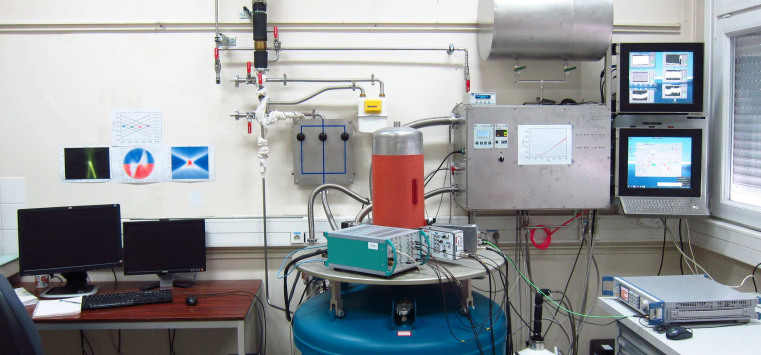
\includegraphics[width=150px]{Images/5_Refrigerateur_Dillution.jpg}
        \caption{Photographie du réfrigérateur à dilution et de l'ensemble du banc de mesure}
    \end{center}
\end{figure}

Pour finir, l'expérience actuelle se déroule actuellement à des températures de 30mK dans un réfrigérateurs à dilution, la température de électronique étant elle de l'ordre de 80mK \cite{10}. Le principe du réfrigérateur à dilution est comparable à celui d'un réfrigérateur classique, des détentes de Joule-Thomsom successives pour refroidir l'hélium à de très basses températures. Le réfrigérateur étant constitué de différents étages dont les températures vont en diminuant pour limiter les pertes. Il faut cependant attendre plusieurs heures pour qu'une température de 30mK soit atteinte.
\section{Vers l'information quantique ?}

L'information quantique se définit comme “la théorie de l'utilisation des spécificités de la physique quantique pour le traitement et la transmission de l'information” \cite{18}. L'utilisation de telles propriétés permettraient d'obtenir des supports et du traitement de l'information bien plus efficaces qu'actuellement.

Bien que l'ordinateur quantique ne soit qu'un but à long (voire très long) terme, la réalisation de transistors de spin à base d'aimants moléculaires est possible. La manipulation et la lecture de spins nucléaires uniques i.e. l'utilisation des propriétés quantiques des aimants moléculaires est permise grâce à des dispositifs comparables à ceux que nous avons utilisés. Ces aimants moléculaires utilisés comme qubits sont ainsi d'excellents candidats pour le stockage de l'information quantique, ils respectent en effet les 5 critères de Divincenzo pour le traitement de l'information quantique.[12] Les critères de Divincenzo définissant quels qubits sont exploitables et assez stables pour effectuer des calculs utiles.
